مدار زیر با ۴ ورودی، \( \text{1IN} \)، \( \text{2IN} \)، \( \text{3IN} \)، \( \text{4IN} \) و ۴ خروجی \( \text{1OUT} \)، \( \text{2OUT} \)، \( \text{3OUT} \)، \( \text{4OUT} \) را در نظر بگیرید.

\begin{enumerate}
	\item 
	جدول صحت\LTRfootnote{\lr{Truth Table}} این مدار را استخراج کنید.
	
	\item 
	با استفاده از جدول کارنو مدار را برای پیاده‌سازی \( \text{POS} \) مستقیماً ساده کنید و سپس آن را دوباره بکشید.
\end{enumerate}



\begin{figure}[h]
	\centering
	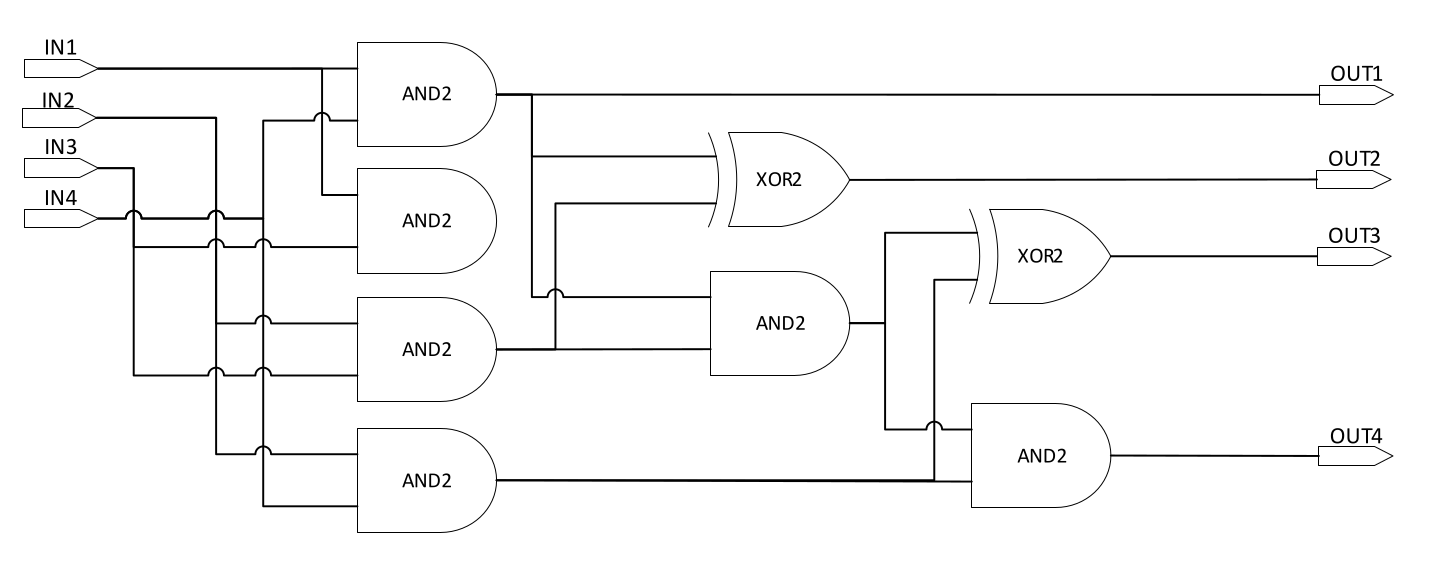
\includegraphics[width=0.9\textwidth]{fig/img2.png}
	\label{img2}
\end{figure}